\chapter{Introduction}
\label{sec:introduction-chapter}

\section{The Capacitated Vehicle Routing Problem}
\label{sec:intro-cvrp-problem}

The Capacitated Vehicle Routing Problem (\textbf{CVRP}), first presented in \textcite{dantzig1959}
under the name of "truck dispatching problem",
is one of the most studied combinatorial optimization routing problem.
The CVRP is an NP-hard (in the strong sense) problem which can be considered a generalization
of the well-known Travelling Salesman Problem (TSP).
The TSP \parencite{flood1956}
is an NP-hard \parencite{garey1976planar} ubiquitous combinatorial optimization problem in the operations research field,
that asks for the determination of a Hamiltonian circuit of minimum cost
\parencite{croes1958, laporte1992,johnson1997,applegate2006,gutin2006,hoffman2013}.
The CVRP can be defined verbally as finding an optimal route for a transportation/distribution/delivery problem
starting from a common point called the depot,
where a homogeneous fleet composed of a fixed number of trucks, subject to capacity constraints,
need to serve customer demands of a single good (i.e. delivery of gasoline to gas stations).
Given as input: a weighted graph representing the road network,
the customer demands and the vehicle capacity,
the problem consists in determining a set of routes, one for each vehicle,
of minimal overall travel distance starting and ending at the depot.
The set of routes need to serve all the customers in the road network exactly once and no more
\parencite{toth2014}.
A diagram showing an example of a CVRP problem along with one of its feasible solution
is provided in \Cref{fig:cvrp-optimal-solution-example}.

\begin{figure}[ht]
	\centering
	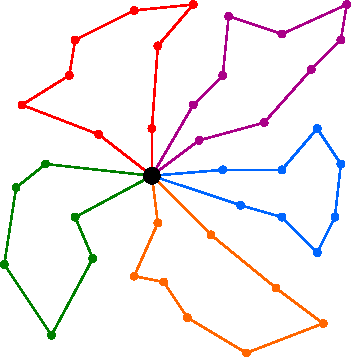
\includegraphics[width=12cm]{Imgs/P-n40-k5-solution.out.cropped.pdf}
	\caption{An example of a feasible solution to a CVRP problem (instance named P-n40-k5).
		There are 39 customers to be served and 5 available trucks with capacity $140$ each. Each color
		represents a different route taken by each truck and the colored dots
		represents the customers served on each route.
		The larger black dot represents the central facility (the depot).
		Credits: \url{http://vrp.galgos.inf.puc-rio.br/index.php/en/plotted-instances?data=P-n40-k5}.
	}
	\label{fig:cvrp-optimal-solution-example}
\end{figure}



Studying effective solution methods for the CVRP may lead to tremendous real-world economic
savings for the management of the provision of goods or services in a distribution system.
Optimal delivery planning can reduce the overall transportation and good costs while
also reducing the waiting time experienced by the customers.
Therefore, studying optimal efficient algorithms and mathematical models for
solving and describing real-world distribution problems,
becomes of vital importance
for the operational management of a cost-efficient planning process \parencite{toth2002,toth2014}.

The CVRP belongs to the wider class of problems known as the Vehicle Routing Problems (VRPs).
There are many variations of VRPs proposed in the literature such as
the Vehicle Routing Problem with Time Windows (VRPTW), and many others.
In the VRPTW \parencite{schrage1981} the vehicles are subject to capacity constraints and
each customer is associated with a time window slot in which it can be served,
Nonetheless, CVRP is the simpler VRP variant to describe,
and yet to this day, it remains the most central and studied routing problem.
For a more complete taxonomy on the many VRP variants refer to \textcite{eksioglu2009, braekers2016}.

While effective (meta)heuristic algorithms have been proposed and applied
successfully to many VRP variants to obtain good-enough solutions
in reduced computation time, in this thesis we are mainly concerned
with exact algorithms for solving the CVRP.
Major contributions employing heuristics for the VRP can be found, among others, in
\textcite{clarke1964, desrochers1989matching, paessens1988savings, foster1976integer}.
Metaheuristics approaches for the VRP can be found, among others, in
\textcite{gendreau1994tabu, cordeau2012parallel, toth2003granular, li2005very, pisinger2007, kytojoki2007efficient, nagata2009,vidal2012, subramanian2013}.
For a more complete survey on (meta)heuristics for the VRP refer to
\textcite{golden1998impact,gendreau2002metaheuristics,gendreau2008,laporte2014chapter,elshaer2020taxonomic}.
Exact algorithms are usually slower than (meta-)heuristics, but given
enough computation time, they can produce a proven optimal solution.
This is achieved by closing the primal-dual bound gap of the objective function.

\medskip

For a fairly complete survey regarding the entire VRP class, we highly suggest
the fairly complete book \citetitle{toth2014} of \textcite{toth2014}.
This book served as a good reference and played a central role
in laying out this introductory chapter.
Other surveys on the matter can be found in the works of \textcite{cordeau2007, baldacci2012, caceres-cruz2015, costa2019}.

\medskip


CVRP is usually defined more rigorously through an Integer Programming (IP) formulation.
The IP formulation is a mathematical optimization tool
which can describe combinatorial optimization problems
through the usage of constraints, usually defined through linear inequalities.
The constraints limit the solution space of the optimization problem.
IP formulations also list a set of decision variables and a linear objective function to be optimized.
In the next section we will provide a more rigorous mathematical
description of the CVRP, and we will present its most commonly employed IP formulations.


\section{Mathematical formulations}
\label{sec:intro-cvrp-mathematical-formulations}

In this section we present the CVRP through some very well known mathematical formulations.
These mathematical formulations are expressed through (Mixed) Integer Programming (MIP, IP)
models.
We present three total mathematical models:

\begin{enumerate}
	\setlength{\itemsep}{0pt}
	\setlength{\parskip}{0pt}

	\item The two-index arc flow formulation \parencite{laporte1983, laporte1985, laporte1986}.
	\item The three-index arc flow formulation \parencite{golden1977}.
	\item The Set Partitioning (SP) formulation \parencite{balinski1964}.
\end{enumerate}

The first two formulations, traditionally designed
for branch-and-cut (\textbf{BAC}) algorithms, employ a polynomial number of variables
but use an exponential number of constraints.
The latter formulation, instead, makes use of a polynomial number of constraints,
but uses an exponential number of variables.
Despite the SP formulation being older, in later years thanks to algorithmic advances
and the development of efficient branch-and-price (\textbf{BAP}) frameworks, it has become the de facto
state-of-the-art core ingredient for solving CVRP problems (see \cite{pessoa2020}).
Another, less common formulation, based on a two-commodity flow description
can be found in \textcite{baldacci2004}.



\subsection{Mathematical notation}
\label{sec:intro-cvrp-mathematical-notation}

Before presenting each formulation we first need to define some basic notation
and mathematical quantities that will be used throughout the remainder of the thesis.

The CVRP is traditionally described as a node routing problem modeled through a symmetric and complete graph theoretical problem,
where: (i) the vertices of the network represent the customers and the depot,
(ii) the edges represent road interconnections.
Let $G = \Tuple*{V, E}$ denote a \textbf{complete undirected network}, where $V = \Set*{0, 1, \dots, N - 1}$ denotes the set of nodes,
$E = \Set*{e = \Set*{i, j} = \Set*{j, i} \mid \allowbreak i,j \in V, \allowbreak i \ne j}$ the set of undirected edges,
and $N$ the total number of nodes in the network.
The value $0 \in V$ is used to denote the depot node.
The edge set $E$ has size $|E|$, which can be computed through combinatorial enumeration: $|E| = \frac{N (N+1)}{2}$.
For convenience, we define $V_0 = V \setminus \Set*{0}$ to express the set of customers,
and $N_0 = N - 1$ to denote the total number of customers.
Let $\delta(S)$ with $S \subseteq V$ denote the edges crossing the set $S$ and its complement $\overline{S} = V \setminus S$.
More formally we can express $\delta(S)$ as $\delta(S) = \Set*{ e = \Set*{i, j} = \Set*{j, i} \in E \mid i \in \Expr*{S \cap V}, j \in \Expr*{ \overline{S} \cap V } }$.
For brevity, we also define $\delta(i) = \delta(\Set*{i})$ to denote the set of edges incident to node $i \in V$.
We also define $E(S) = \Set*{e = \Set*{i, j} = \Set*{j, i}\in E \mid i, j \in S}$ to denote the set of edges having both end points in set $S \subseteq V$.

Let $q_{i} \in \R,\ q_{i} \ge 0 \quad \forall i \in V$ denote the demand function, which represent the required demand that need to be served for vertex $i \in V$.
For convenience, we fix a fictitious demand for the depot: $q_0 = 0$.
Given a set $S \subseteq V$, we define $q(S) = \sum_{i \in S} q_i$ as the total demand of the set $S \subseteq V$.
Let $c_{ij} \in \R, c_{ij} > 0$ denote the distance function between a pair of nodes  $i, j \in V$.
The loop arcs $\Set*{i, i} \notin E$ in CVRP are traditionally not allowed, thus we fix $c_{ii} = \infty$.
We assume a Euclidean CVRP problem, i.e. the distance function is symmetric $c_e = c_{ij} = c_{ji}$ and satisfies the triangle inequality $c_{ij} \le c_{ih} + c_{hj}$.
We are also given the total number of identical trucks $K \in \N_+$ and an upper bound $Q \in \R_+$ representing the capacity of each truck.
For convenience of notation, we also define $\mcK = \Set*{1, \dots, K}$ to denote the set of trucks.
Given a set $S \subseteq V_0$, we denote by $r(S)$ as the minimum number of vehicles required to serve all customers $i \in S$.
The value of $r(S)$ can be obtained by solving an NP-hard Bin Packing Problem associated with the CVRP and set $S$.
As we will see later, it is often simpler to link $r(S)$ to the trivial lower bound of the Bin Packing Problem \parencite{martello1990}:

\begin{equation}
	r(S) \ge \ceil*{\frac{q(S)}{Q}}
\end{equation}

A route $p$ is a loop-back sequence $p = \Tuple*{p_0, p_1, \dots, p_u, p_{u + 1}}$,
with $p_0 = p_{u + 1} = 0$
in which $\Set*{p_1, \dots, p_u} \subseteq V_0$ customers are visited.
The route $p$ has a travel cost of $c_p = c(p) = \sum_{i=0}^{u} c_{p_i,p_{i+1}}$
with resource consumption $q_p = q(p) = \sum_{i=0}^{u} q_{i}$.
A feasible solution to a CVRP problem consists of \textbf{exactly} $K$ routes (or circuits)
associated with each vehicle starting and ending at the depot node.
The traditional definition of CVRP requires full use of the total number of available vehicles $K$,
however,
this requirement can lead to suboptimal solutions with respect to using fewer vehicles for some cases.
In classic CVRP, each customer is visited exactly once (elementarity condition),
and the sum of the customer demands visited in each tour does not exceed the vehicle capacity $q(p) \le Q$.
An optimal solution to the CVRP is a feasible solution which minimizes the sum of the overall edge weights across all the tours.

\medskip

The TSP can be considered a special case of CVRP where $Q \ge q(V)$ and $K = 1$.
Therefore, all the relaxations and many results obtained for the TSP are valid, or at least extendable, to the CVRP.

\medskip

Some variants of the basic version of the CVRP, not considered in this thesis, allows using only a subset of the total available vehicles,
or consider a heterogeneous fleet characterized by different capacities $Q_1, \dots, Q_k$.
In the remainder of this section we introduce the two most common IP mathematical formulations for the classical version of the CVRP.

\subsection{The two-index arc flow formulation}
\label{sec:intro-cvrp-two-index-flow-formulation}

The two-index arc flow formulation (2F) was first presented in \cite{laporte1983, laporte1985} for the symmetric case,
and later generalized to the undirected case in \cite{laporte1986}.

The two-index arc flow formulation is traditionally tackled with branch-and-cut frameworks.
We define a set of integer variables $x_e \in \Set*{0, 1, 2}$ to indicate the number of times
a vehicle traverses edge $e = \Set*{i, j} = \Set*{j, i} \in E$ in the optimal solution.
There are $O(N^2)$ number of integer variables in the model.
The two-index arc flow formulation can be described as an Integer Programme (IP):

\begin{align}
	\min_{x} \quad z_\mt{2F}(x) & = \sum_{e \in E} c_e x_e \label{eq:two-index-flow-obj-func}                                                                                        \\
	                            & \sum_{e \in \delta(i)} x_e = 2                              & \quad \forall i \in V_0 \label{eq:two-index-flow-two-edges-incident-per-customer}    \\
	                            & \sum_{e \in \delta(0)} x_e = 2 K                            & \label{eq:two-index-flow-two-k-edges-incident-in-the-depot-node}                     \\
	                            & \sum_{e \in \delta(S)} x_e \ge 2 r(S)                       & \quad \forall S \subseteq V_0,\ |S| \ge 1 \label{eq:two-index-flow-ccc}              \\
	                            & x_e                   \in \Set*{0, 1, 2}                    & \quad \forall e \in \delta(0) \label{eq:two-index-flow-x-mip-var-bounds-depot}       \\
	                            & x_e                   \in \Set*{0, 1}                       & \quad \forall e \in E \setminus \delta(0) \label{eq:two-index-flow-x-mip-var-bounds}
\end{align}

where $z_\mt{2F}(x)$, as defined in \eqref{eq:two-index-flow-obj-func}, is the objective function meant to minimize the overall routing cost (travel time).
Constraint \eqref{eq:two-index-flow-two-edges-incident-per-customer} is the degree constraint which imposes flow conservation: exactly two incident edges must be picked for each customer.
Constraint \eqref{eq:two-index-flow-two-k-edges-incident-in-the-depot-node}, is the degree constraint at the depot, it forces that exactly $2K$ incident edges at the depot are picked, thus forcing exactly $K$ routes to be constructed.
Constraints \eqref{eq:two-index-flow-x-mip-var-bounds-depot} and \eqref{eq:two-index-flow-x-mip-var-bounds} forces each edge to be traversed at most once,
except for all edges incident at the depot.
The edge-case modeled in constraint \eqref{eq:two-index-flow-x-mip-var-bounds-depot} is necessary to allow single-customer routes.
Constraint \eqref{eq:two-index-flow-ccc}, are the so-called Capacity Cut Constraints (CCC), also called Rounded Capacity Constraints (RCC), they function both:
(i) as Subtour Elimination Constraints (SECs), by imposing connectivity of the solution by avoiding the formation of spurious unconnected subtours,
and (ii) as a capacity constraint, by imposing that any customer set $S$ is crossed by a number of edges not smaller than $r(S)$.
Recall that, $r(S)$ represents the minimum number of vehicles needed to serve all customers in set $S$,
also, $r(S)$ always satisfies $r(S) \ge 1$ for non-trivial CVRP instances: $q(S) > 0$.

It was shown in \textcite{martello1990knapsack, cornuejols1993}, that it is possible to replace $r(S)$ in constraint
\eqref{eq:two-index-flow-ccc}, with the much simpler Bin Packing Problem lower bound $\ceil*{q(S) / Q}$
thus obtaining the following inequality:

\begin{equation}
    \label{eq:two-index-flow-ccc-bpp-lb}
	\sum_{e \in \delta(S)} x_e \ge 2 \ceil*{\frac{q(S)}{Q}}   \quad \forall S \subseteq V_0, |S| \ge 1
\end{equation}

The looser inequality of \cref{eq:two-index-flow-ccc-bpp-lb} is sufficient to optimally solve
the two-index arc flow formulation.
Although, a better lower bound for the Bin Packing Problem can improve the linear
relaxation, thus reducing the number of branching occurrences.

The CCC constraints in \cref{eq:two-index-flow-ccc}, may be transformed in the so called Generalized Subtour Elimination Constraints (GSEC) \parencite{laporte1985},
by means of the degree constraints of \cref{eq:two-index-flow-two-edges-incident-per-customer,eq:two-index-flow-two-k-edges-incident-in-the-depot-node}:

\begin{equation}\label{eq:cvrp-2flow-gsec}
	\sum_{e \in E(S)} x_{ij} \le |S| - r(S) \quad \forall S \subseteq V_0,\ |S| \ge 1
\end{equation}

where, again, $r(S)$ may be replaced by the trivial Bin Packing Problem lower bound $\ceil*{q(S) / Q}$.

The GSEC avoid the formation of spurious unconnected subtours and impose that at least $r(S)$ edges leave set $S$.
The number of GSEC (or CCC) inequalities appear in exponential number in the two-index formulation model,
thus making a direct solution of the linear relaxation impractical.
To overcome this issue, it is possible to avoid adding the GSEC inequalities statically in the model.
Instead, an appropriate cutting-plane algorithm and separation procedure may be employed to generate dynamically
only the necessary (violated) GSECs constraints
during the running time of the branch-and-cut algorithm,

Another approach is to avoid the usage of the exponential number of SECS entirely.
This is the approach taken by the so-called compact models (see \cite{miller1960, christofides1979vehicle, desrochers1991}).
These models make use of a polynomial number of constraints.
Unfortunately these compact formulations are known to produce significantly weaker linear relaxations.
In fact, it has been mathematically proven,
that the SECs are very strong for the TSP: they are facet-defining for the polytope;
i.e. they uniquely characterize the convex-hull \parencite{grotschel1975}.
However, similar mathematical proofs cannot be extended to the CVRP,
since due to the more complex structure of this generalized problem,
little satisfactory results have been obtained in studying the polyhedral characteristics
for even the standard variation of the VRP, see \textcite{campos1991, cornuejols1993}.

Unfortunately, as it was proven in \textcite{augerat1995} the separation problem
for the capacity cut constraints is NP-complete, thus limiting the applicability
of this formulation for solving the CVRP.
For this reason, some authors \parencite{augerat1995, augerat1998, ralphs2003} designed
several fractional separation heuristics for the CCC.
However,
an exact CCC separation is required for integral solutions
to ensure the correctness of the optimal solution.
\textcite{lysgaard2003cvrpsep} implements efficient
heuristics for separating the CCC of \cref{eq:two-index-flow-ccc}.


\subsection{The three-index arc flow formulation}
\label{sec:intro-cvrp-three-index-flow-formulation}

When modeling more "colorful" variations of the CVRP,
the two-index arc flow model falls short in providing sufficient descriptive power.
For example,
the simple CVRP variant where the fleet of trucks is heterogeneous
and characterized by capacities $Q_1, \dots, Q_K$,
cannot be described with the two-index arc flow formulation,
since there's no clear one-to-one mapping on which truck crosses an edge $e \in E$.

The three-index arc flow formulation (3F),
first presented in \textcite{golden1977},
fixes this issue.
The 3F formulation makes use $O(N^2 K + N K)$ integer variables.
A set of integer variables $x_{ek} \in \Set*{0, 1, 2},\ e = \Set*{i, j} \in E,\ k \in \mcK$
is used to encode the number of times a truck $k$ traverses an edge $e \in E$.
Another set of binary variables $y_{ik} \in \Set*{0, 1},\ i \in V,\ k \in \mcK$
is used to model whether truck $k$ covers a node $i \in V$.


The three-index arc flow formulation can be described as an Integer Programme (IP):


\begin{align}
	\min_{x, y} \quad z_\mt{3F}(x, y) & = \sum_{k \in \mcK} \sum_{e \in E} c_{e} x_{ek} \label{eq:three-index-flow-obj-func}                                                                                                                           \\
	                                  & \sum_{k \in \mcK} y_{ik} = 1                                                         & \quad \forall i \in V_0                                              \label{eq:three-index-flow-all-customers-visited}  \\
	                                  & \sum_{k \in \mcK} y_{0k} = K                                                         & \label{eq:three-index-flow-tour-starts-and-ends-at-depot}                                                               \\
	                                  & \sum_{e \in \delta(i)} x_{ek} = 2 y_{ik}                                             & \quad \forall i \in V,\ \forall k \in \mcK \label{eq:three-index-flow-force-visited-customer-if-flow}                   \\
	                                  & \sum_{i \in V} q_i y_{ik} \le Q                                                      & \quad \forall k \in \mcK \label{eq:three-index-flow-force-resource-upper-bound}                                         \\
	                                  & \sum_{e \in \delta(S)} x_{ek} \ge 2 y_{hk}                                           & \quad \forall h \in S,\ \forall S \subseteq V_0,\ |S| \ge 2,\ \forall k \in \mcK \label{eq:three-index-flow-secv1}      \\
	                                  & x_{ek}                   \in \Set*{0, 1, 2}                                          & \quad \forall e \in \delta(0),\ \forall k \in \mcK             \label{eq:three-index-flow-x-mip-var-bounds-depot}       \\
	                                  & x_{ek}                   \in \Set*{0, 1}                                             & \quad \forall e \in E \setminus \delta(0),\ \forall k \in \mcK             \label{eq:three-index-flow-x-mip-var-bounds} \\
	                                  & y_{ik}                    \in \Set*{0, 1}                                            & \quad \forall i \in V,\ \forall k \in \mcK  \label{eq:three-index-flow-y-mip-var-bounds}
\end{align}

where $z_\mt{3F}(x, y)$, as defined in \eqref{eq:three-index-flow-obj-func}, is the objective function to be minimized (i.e. the overall travel distance).
Constraint \eqref{eq:three-index-flow-all-customers-visited} forces all customers to be served exactly once.
Constraint \eqref{eq:three-index-flow-tour-starts-and-ends-at-depot} forces all the truck tours to start at the depot and end at the same spot.
Constraint \eqref{eq:three-index-flow-force-visited-customer-if-flow} binds the $y_{ik}$ variables to the corresponding $x_{ijk}$ variables, by ensuring that if a truck's route passes through a vertex, then the corresponding node is marked as visited.
Constraint \eqref{eq:three-index-flow-force-resource-upper-bound} is the capacity upper bound constraint and it ensures that the demand served by each truck does not exceed the truck capacity.
Constraints \eqref{eq:three-index-flow-secv1} are the Generalized Subtour Elimination Constraints (GSECs), they impose the connectivity of the route and are used to avoid the formation of spurious unconnected subtours.
Constraints \eqref{eq:three-index-flow-x-mip-var-bounds-depot} and \eqref{eq:three-index-flow-x-mip-var-bounds} forces each edge to be traversed at most once,
except for all edges incident at the depot.
The edge-case modeled in constraint \eqref{eq:three-index-flow-x-mip-var-bounds-depot}
is necessary to allow single-customer routes.
Finally, constraint \eqref{eq:three-index-flow-y-mip-var-bounds}
bounds and forces integrality for the $y_{ik}$ binary variables.

Constraint \eqref{eq:three-index-flow-secv1} may be replaced in an equivalent form
with traditional (non generalized) TSP subtour elimination constraints (see \textcite{fisher1981}):

\begin{equation}\label{eq:three-index-flow-secv2}
	\sum_{e \in E(S)} x_{ek} \le |S| - 1 \quad \forall S \subseteq V_0, |S| \ge 2,\ \forall k \in \mcK
\end{equation}

Since the number of (G)SECs is exponential in the number of nodes $N$, they are usually not inserted statically in the model but are generated lazily within the running time of the resolution process.

The three-index arc flow model generalizes the two-index version.
In fact, the two-index arc flow model may be viewed as a special case of the three-index by aggregating
all $x_{ek}$ into a single variable $x_e$:


\begin{equation}
	x_e = \sum_{k \in \mcK} x_{ek} \quad \forall e \in E
\end{equation}

However, the three-index arc flow formulation suffers a major downside compared to the two-index version.
When modeling homogeneous fleets CVRPs the 3F model suffers from a multiplicity of the solution space.
In fact, since all the vehicles share the same capacity,
new feasible solutions can be obtained through symmetry by simply permuting the identity $k \in \mcK$ of each truck.


\subsection{The Set Partitioning (SP) formulation}
\label{sec:intro-set-partition-formulation}

The Set Partitioning (SP) formulation,
sometimes also called Path Flow formulation,
is an extended formulation, which was originally presented in \textcite{balinski1964}.
It works substantially differently from the two/three-index arc flow formulation
or many other commonly encountered IP models.
The SP formulation uses a very small number of constraints
while offloading much of the search-space complexity to an exponential number of binary variables.


The SP formulation can be viewed as a Dantzig-Wolfe decomposition \parencite{dantzig1960}
and commodity aggregation \parencite{desaulniers1998}
of the three-index arc flow formulation.
The Dantzig-Wolfe reformulation approach is an application of a
decomposition principle where one chooses to solve many smaller sizes
structured sub-problems instead of being confronted to
the original problem resolution complexity are beyond what can be
solved in reasonable time \parencite{vanderbeck2005}.
Let $P = \Set*{p \mid p\ \text{is a single-truck feasible route}}$ be the set of all feasible routes.
Let $\lambda_p \in \Set*{0, 1}$ be a binary variable indicating whether route $p$ is selected.
Let $a_{ip}, a_{ep} \in \Z$ be "static encodings" (integer coefficients)
for a route $p \in P$ that respectively count
the number of times vertex $i \in V$ or an edge $e \in E$ is covered.

We recall that $c_p = c(p)$ represents the cost of a feasible route $p \in P$,
which can be trivially computed in $O(N)$.
The SP model forces $K$ routes $\Tuple*{p_1, \dots, p_K} \in P^K$ to be included in the optimal solution.

The SP formulation is described through an Integer Programme (IP):


\begin{align}
	\min_{\lambda} \quad z_\mt{SP}(\lambda) & = \sum_{p \in P}  c_p \lambda_p \label{eq:set-partitioning-obj-func}                                                                                                                                           \\
	                                        & \sum_{p \in P} \lambda_{p} = K\label{eq:set-partitioning-K-routes}                                                                                                                                             \\
	                                        & \sum_{p \in P}  a_{ip} \lambda_p = 1                                 & \quad \forall i \in V_0                                              \label{eq:set-partitioning-customers-visited-by-exactly-one-route} \\
	                                        & \lambda_p                    \in \Set*{0, 1}                         & \quad \forall p \in P \label{eq:set-partitioning-lambda-mip-var-bounds}
\end{align}

where, $z_\mt{SP}(\lambda)$, as defined in \eqref{eq:set-partitioning-obj-func} is the objective function to be minimized (i.e. the overall travel distance).
Constraint \eqref{eq:set-partitioning-customers-visited-by-exactly-one-route} forces each customer to be covered by exactly one route.
Constraint \eqref{eq:set-partitioning-K-routes} enforces that exactly $K$ routes are selected.
Finally, constraint \eqref{eq:set-partitioning-lambda-mip-var-bounds} is the bounding and integrality constraints for binary variables $\lambda_p \ \forall p \in P$.

As one may guess,
due the exponential number of binary variables,
the SP formulation cannot be instantiated nor directly solved.
However,
a variant of the SP formulation can be tackled efficiently by Column Generation (CG) approaches
embedded inside a branch-and-price (BAP) framework.
Branch-and-price frameworks and column generation have been applied
with high success to the vehicle routing problems.


As, \textcite{toth2002} point out, if the distance matrix satisfies the triangle inequality,
than it is possible to rewrite the SP formulation into a totally equivalent Set Covering (SC) formulation
by substituting \cref{eq:set-partitioning-customers-visited-by-exactly-one-route} in favor of the simpler inequality:

\begin{equation}\label{eq:set-covering-customers-visited-by-exactly-one-route}
	\sum_{p \in P}  a_{ip} \lambda_p \ge 1  \quad \forall i \in V_0
\end{equation}

The set of feasible paths $p \in P$ in the SC formulation
become all non-elementary routes that respect the vehicle capacity.
Under the triangle inequality assumption,
any feasible solution for the SP formulation is also feasible for the SC formulation.
Transforming the SP to the SC formulation vastly shrinks (halves) the size of the dual solution space.

\medskip


The SP formulation has two main advantages.
First, its linear relaxation provides excellent lower bounds \parencite{bramel1997},
compared to the two or three arc flow formulation.
Second, it can handle many VRP variants,
even described through very complex constraints,
since their definitions are captured within the definition of the set $P$ itself.


\medskip

In the next sections we will introduce
the branch-and-price (BAP) framework and the Column Generation (CG) approach,
key components employed in contemporary CVRP solvers.
Refer to \textcite{vanderbeck2005, lubbecke2005} for a review on column generation
approaches to solve generic MIP problems.


\section{Branch and Price}
\label{sec:intro-branch-and-price}

Branch-and-price (BAP) frameworks are in essence a branch-and-bound (BAB) scheme \parencite{land2010},
i.e. making use of a search tree,
that originates when solving the SP formulation for vehicle routing problems.
Compared to more traditional branch-and-cut (BAC) frameworks,
their primary focus is the usage of a Column Generation (CG) technique for improving the dual bound,
see \textcite{righini2008}.
BAP frameworks were first applied successfully in \textcite{gilmore1961} to the Cutting-Stock problem.
For a primer introduction to branch-and-price schemes refer to the work of \textcite{barnhart1998}.
An extension of the BAP framework, the so-called branch-price-and-cut (BPC) framework,
is in essence a branch-and-bound (BAB) algorithm where dual bounds are obtained through column generation (CG)
and cutting-planes are added to strengthen the linear relaxations associated to each node of the search-tree.

In the next section we will illustrate the column generation algorithm
and the pricing problem, two vital pieces in branch-and-price frameworks.
We refer the reader to \textcite{feillet2010}, which contains a tutorial
on column generation and branch-and-price algorithms.
Other more useful more in-depth references about column generation can be found in \textcite{desrosiers2005, lubbecke2005}.
For a more problem-independent introduction in branch-price-and-cut frameworks refer to \textcite{desrosiers2011}.


\subsection{Column generation and the Pricing Problem}
\label{sec:column-generation-and-pricing-problem}

Consider the \textbf{Master Problem} (MP) defined
as the linear relaxation of the SP formulation obtained by relaxing the integrality constraints:

\begin{align}
	\min_{\lambda} \quad z_\mt{MP}(\lambda) & = \sum_{p \in P}  c_p \lambda_p \label{eq:mp-obj-func}                                                                                                                             \\
	                                        & \sum_{p \in P} \lambda_{p} = K\label{eq:mp-K-routes}                                                                                                                               \\
	                                        & \sum_{p \in P}  a_{ip} \lambda_p = 1                   & \quad \forall i \in V_0                                              \label{eq:mp-customers-visited-by-exactly-one-route} \\
	                                        & 0 \le \lambda_p \le 1                                  & \quad \forall p \in P \label{eq:mp-lambda-mip-var-bounds}
\end{align}


The constraint $\lambda_p \le 1$ in \cref{eq:mp-lambda-mip-var-bounds} is implied from \cref{eq:mp-customers-visited-by-exactly-one-route} and can thus be removed.
An optimal solution to the MP provides a valid dual bound at the root node of the search tree.
The master problem can be modified by adding cuts or branching constraints to improve the obtained dual bound.

The dual problem associated with \labelcref{eq:mp-obj-func,eq:mp-customers-visited-by-exactly-one-route,eq:mp-K-routes,eq:mp-lambda-mip-var-bounds}
is:

\begin{align}
	\max_{\pi} \quad z_\mt{DMP}(\pi) & =  K \pi_0 + \sum_{i \in V_0} \pi_i \label{eq:dmp-obj-func}                                                    \\
	                                 & \pi_0 + \sum_{i \in V_0} a_{ip} \pi_i \le c_p               & \quad \forall p \in P \label{eq:dmp-constraint1} \\
	                                 & \pi_0 \in \R &  \label{eq:dmp-constraint2} \\
	                                 & \pi_i \in \R &  \quad \forall i \in V_0 \label{eq:dmp-constraint3}
\end{align}

where $\pi_0 \in \R, \pi_i \in \R \quad \forall i \in V_0$ represents the dual variables
associated respectively with constraints \labelcref{eq:mp-K-routes,eq:mp-customers-visited-by-exactly-one-route}.
In case the Set Covering formulation is used \cref{eq:dmp-constraint3} can be replaced in favor of $\pi_i \ge 0 \quad \forall i \in V_0$,
thus reducing the dual solution space.
When solving the MP,
at each iteration of the simplex algorithm \parencite{dantzig1955} we seek for a non-basic variable (i.e. column)
to price out and enter the basis.
This is achieved by evaluating the dual variables $\pi \in \R^N$.
Due to the huge size of the set of routes $P$,
it is computationally intractable to evaluate numerically the dual variables $\pi \in \R^{N}$.

\medskip

Therefore, in BAP frameworks we consider only a small subset of columns $\mcP \subseteq P$,
obtaining the following linear program:

\begin{align}
	\min_{\lambda} \quad z_\mt{RMP}(\lambda) & = \sum_{p \in \mcP}  c_p \lambda_p \label{eq:rmp-obj-func}                                                                                                                              \\
	                                         & \sum_{p \in \mcP} \lambda_{p} = K\label{eq:rmp-K-routes}                                                                                                                                \\
	                                         & \sum_{p \in \mcP}  a_{ip} \lambda_p = 1                    & \quad \forall i \in V_0                                              \label{eq:rmp-customers-visited-by-exactly-one-route} \\
	                                         & \lambda_p \ge 0                                            & \quad \forall p \in \mcP \label{eq:rmp-lambda-mip-var-bounds}
\end{align}

which takes the name of \textbf{Restricted Master Problem} (RMP).

In BAP frameworks, we seek to solve the following sub-problem:

\begin{equation}\label{eq:pp-problem}
{c^\star_p} = \min_{p \in P} \Set*{ \bar{c}_p = \sum_{e = \Set*{i, j} \in E} \Expr*{c_{e} - \frac{\pi_i + \pi_j}{2}} a_{ep}  }
\end{equation}

which takes the famous name of \textbf{Pricing Problem} (PP).
In \cref{eq:pp-problem}, $\bar{c}_p$ denotes the reduced cost of a route $p \in P$
and $c^\star_p$ is the reduced cost of the optimal route $p^\star \in P$
that leads to the best dual bound improvement.
Notice that $\bar{c}_p$ can also be expressed as $\bar{c}_p = c_p - \pi_0 - \sum_{i \in V_0} \pi_i a_{ip}$.
For convenience,
we define $\bar{c}_{e} = c_{e} - \frac{\pi_i + \pi_j}{2}$
as the reduced cost of an edge $e\in E$.

Any $p \in P$ which satisfies $\bar{c}_p < 0$ is a valid column which can enter the basis of the RMP.
The BAP solver needs to smartly manage the set $\mcP \subseteq P$, which it stores it inside a pool.
It is responsibility of the BAP framework to efficiently manage which routes
to preserve or drop from $\mcP$ during the running time of the resolution process.
Due to the high sparseness of the set $\mcP$, any $p \in \mcP \mid \lambda_p = 0$
is a valid candidate that may be dropped from the pool.
A BAP framework must be engineered correctly as to maintain
the size of the pool $\mcP \subseteq P$ manageable.

\medskip

The resolution method, or algorithm,
used to solve the PP is usually called \textbf{oracle} or \textbf{pricer} in the literature.
The oracle needs to solve the pricing sub-problem which, due to the definition of the set $P$,
coincides with solving an Elementary Shortest Path Problem with Resource Constraints (ESPPRC)
over a \textbf{new directed symmetric} network with weights
$\bar{c}_{ij} = c_{ij} - \frac{1}{2} \pi_i - \frac{1}{2} \pi_j$.
Resources are non-decreasing quantities,
such as capacity or time,
which are used to evaluate
the feasibility of a route.
The ESPPRC problem asks for an elementary path (i.e. each vertex visited at most once) starting
from a vertex, called a source vertex, and ending in another vertex, called the sink vertex.
In the ESPPRC, the depot node is split in two vertices (one source, one sink)
and the newly obtained network is characterized by $N + 1$ vertices.

\medskip

The column generation (CG) is an iterative algorithm,
successfully applied to a wide variety of problems \parencite{desrosiers2005},
which alternates between two phases \parencite{desaulniers2018}:
\begin{enumerate}
	\setlength{\itemsep}{0pt}
	\setlength{\parskip}{0pt}

	\item The simplex algorithm for solving the RMP, which is characterized by one or more pivot operations.
	\item One or several iterations of the Pricing Problem (PP) solved by invoking the pricer algorithm.
	      The simplex algorithm invokes the pricer to verify whether other pivot operations
	      can be performed for improving the dual bound.
	      The pricer algorithm usually lives in a separate external code module from the branch-and-price code.
\end{enumerate}

The column generation may also be interpreted as a cutting-plane strategy
for the dual problem.
The column generation procedure stops mainly under two scenarios:
(i) when no more negative reduced cost routes exist,
i.e. the PP outputs a $p^\star$ achieving $c^\star_p \ge 0$,
(ii) the CG procedure tails off,
i.e. the gained dual bound improvements
compared to the running time to generate a column
become suboptimal (optional).

If after the column generation procedure
the candidate solution to the RMP $\lambda^*$ satisfies the integrality constraints,
$\lambda^\star_p \in \Set*{0, 1} \quad \forall p \in \mcP$,
no branching or cutting planes are required,
and the candidate solution $\lambda^*$ can be used to update the incumbent.
If, instead,
$\exists p \in \mcP \mid \lambda^\star_p \notin \Set*{0, 1}$
then a branching strategy is usually necessary
in order to seek for the best integral solution.
When all the nodes of the branch-and-bound tree have been explored or pruned,
then the CVRP problem is solved to optimality
and the current incumbent solution becomes the optimal solution
$(p_1, \dots, p_K) \mid \lambda^\star_{p_i} = 1$.

\medskip

It is also important to note,
that the CG doesn't need to solve the PP optimally at each iteration of the simplex algorithm.
To improve the dual bound,
it is usually enough to find any $p \in P$ achieving $\bar{c}_p < 0$.
There is no need to solve the pricing problem exactly,
except to prove the optimality at the last column generation iteration.
Therefore, fast and efficient heuristic algorithms may be employed
to tackle the pricing problem,
especially during the very first few pricing iterations,
where finding good reduced cost columns is surprisingly easy.

\medskip

In this thesis, we will mostly analyze the CVRP problem under the SP formulation.

\subsection{Branching, Route Enumeration and Cut Generation}
\label{sec:intro-branching-and-cut-generation-within-bap-frameworks}

In order to satisfy the integrality constraints for the SP formulation,
solving the RMP at the root node is almost always not enough.
The CG algorithm may in fact terminate with a non-zero duality gap.
Therefore,
a search-tree and a branching scheme is employed
to seek for the optimal integral solution $\lambda^\star_p \in \Set*{0, 1} \quad \forall p \in P$.

Although non strictly-necessary, modern BAP also use
cut generation procedures to efficiently improve the dual bound and the convergence speed.
Modern BAP frameworks
are in fact a hybridization between a BAP and a BAC framework,
making them a branch-price-and-cut (BPC) frameworks.
Some notable works integrating cutting-planes and proposing
a BCP approach for the VRP can be found \textcite{fukasawa2006, ropke2012}.
Refer to \textcite{sadykov2019modern} for a discussion of the state-of-the-art
components that are part of modern branch-and-price frameworks.

\medskip

It is important to note however that branching is not a strictly required operation.
Route enumeration is another technique that can be used in place of branching
for obtaining integral solutions which was first proposed for the CVRP in \textcite{baldacci2008}.
In route enumeration, all elementary routes that may belong to the VRP optimal solution are enumerated,
and an SP formulation containing all these enumerated routes are solved through a MIP.
Route enumeration is obtained through a labeling algorithm similar to the one employed in the pricing problems.
The problem of this approach is the possibly huge number of routes that needs to be enumerated,
and this quantity is highly linked to the tightness of the duality gap,
and with the average length of a tour $N / K$.
Route enumeration is an operation that takes exponential space complexity,
but it can drastically improve the performance of the BPC on some instances.
The major contributions employing route enumeration in place of branching can be found in
\textcite{baldacci2008,baldacci2011}.

Modern BPC frameworks instead take a hybrid approach by combining branching and route enumeration
(see \cite{pessoa2008, pessoa2009,contardo2014,pecin2017improved,pecin2017new,pessoa2020}).
After the convergence of the column generation, route enumeration is attempted.
If the number of enumerated routes starts to exceed a maximum limit, enumeration
is preemptively aborted and conventional branching is applied.
Once the primal-dual bound gap $\bar{z} - \ubar{z}$ reaches desirable levels, the route enumeration
procedure will enumerate all routes under the maximum limit.
At the point the associated RMP formulation can be solved efficiently through a MIP.

We will not concentrate much of our attention on route enumeration in this
thesis, since their presence doesn't influence the pricing problem.
Nonetheless, it's important to know about its existence and role within
the branch-and-price frameworks.

\medskip

Branching and cut generation in BCP frameworks are more delicate operations
compared to more traditional BAC frameworks due to the presence of the pricing problem.
As classified in \textcite{dearagao2003},
depending on the branching and cut generation schemes employed,
two classes of inequalities are possible:
\textbf{robust} versus \textbf{non-robust} inequalities.

A \textbf{robust} inequality is an inequality
which can be safely added to the RMP
without altering the structure of the set of feasible paths $P$ \parencite{fukasawa2006}.
That is,
robust inequalities do not require explicit modeling in the PP formulation
and instead manifest their contribution directly in the reduced cost edges $\bar{c}_e$.
An oracle, therefore,
after the introduction of a robust inequality in the RMP,
needs to solve the same ESPPRC problem but with slightly different weights associated on each edge.

A \textbf{non-robust} inequality, instead,
is much harder to handle since it changes the structure of the set of feasible paths $P$.
Non-robust inequalities may in general have great potential at reducing the integrality gap
but,
unfortunately, require explicit modeling and support from the oracle.
These types of inequalities can drastically complicate the pricing problem,
trading better dual bound improvements for increased column generation times.
Therefore, their usage must be assessed on a case-by-case basis \parencite{desaulniers2011}.
Non-robust inequalities may present themselves both in the branching and cut-generation phases.

In this thesis
we will mostly concentrate on branching and cut generation schemes
which make use of \textbf{robust} inequalities.
Refer to \textcite{desaulniers2011} for an introduction in cutting planes for BAP algorithms.


\begin{comment}
    \textcite{lubbecke2005}
The purpose of the RMP (as is the purpose of subgradient algorithms in Lagrangian relaxation) is to
provide dual variables: To be transferred to the subproblem, and to control our stopping criterion. In
the end only, we have to recover from the RMP a primal feasible solution to the compact formulation.
Primal methods, like column generation, maintain primal feasibility and work towards dual feasi-
bility. It is therefore only natural to monitor the dual solution in the course of the algorithm. In our
opinion, the dual point of view reveals most valuable insight into the algorithm’s functioning. We call
the polyhedron associated with the dual of the RMP the dual polyhedron. A dual solution to the RMP
needs not be unique, e.g., if the primal is degenerate. This is significant inasmuch the dual solution di-
rectly influences the selection of new columns. Since a dual basic solution corresponds to an extreme
point of the optimal face, it may be a bad representative of all the dual solutions obtainable.
\end{comment}

\subsubsection{Branching}
\label{sec:bap-branching}

In this section we will introduce branching for the SP formulation,
under the assumption that a branch-and-price scheme is employed
for solving the CVRP.

At first glance,
it might seem reasonable to branch directly on the $\lambda_p$ variables of the SP formulation.
Unfortunately, such form of branching has two main problems \parencite{vanderbeck2010reformulation}.
First, it is non-robust and leads to a harder pricing problem: an ESPPRC with forbidden paths \parencite{villeneuve2005}.
Second, it produces a highly unbalanced tree.

Most of the branching approaches studied in the literature for the CVRP involve
mere extension of branching schemes used traditionally for the TSP.
In fact, one of the most simple branching scheme,
yet one of the most effective,
involves \textbf{branching on edges}.
The branching on edges scheme was first proposed for the CVRP in \textcite{christofides1969},
and later re-adapted in different forms in \textcite{fisher1994, miller1995}.
The arc flows can be easily computed from the master problem as:

\begin{equation}
	x_e = \sum_{p \in P} a_{ep} \lambda_p  \quad \forall e \in E
\end{equation}

where $a_{ep}$ represents the number of times route $p \in P$ crossed edge $e \in E$.

Given a candidate fractional solution $\lambda^\star_p \quad \forall p \in \mcP$
and a valid edge $e$ to branch on, $e \mid x_e \notin \Set*{0, 1, 2}$,
it is possible to generate two descendant nodes in the search tree
to continue scanning for integral solutions:

\begin{equation}\label{eq:sp-branching-on-arcs}
	x_e \le \floor*{\sum_{p \in \mcP} a_{ep} \lambda^\star_p}, \quad
	x_e > \ceil*{\sum_{p \in \mcP} a_{ep} \lambda^\star_p}
\end{equation}

Branching on arcs is an approach which is both: extremely simple and robust.
Let $\omega_e \in \R$ represent the dual variable associated to
edge $e \in E$ and to
one of the branching polarity in \cref{eq:sp-branching-on-arcs},
then, after branching,
the new reduced cost $\bar{c}_e$ for an arc $e \in E$ becomes:

\begin{equation}
\bar{c}_e = c_e - \frac{\pi_i + \pi_j}{2} - \omega_e
\end{equation}

where again $\pi \in \R^N$ represents the dual variables associated with \cref{eq:mp-K-routes,eq:mp-customers-visited-by-exactly-one-route}.

Branching on edges has the disadvantage of achieving only local changes
to the fractional solution.
For this reason, \textcite{augerat1998} propose an
approach to obtain larger perturbations.
They achieve this by branching on Rounded Capacity Constraints (RCCs) defined over
an arbitrary set $S \subseteq V_0$ with two descendant nodes:
\begin{equation}\label{eq:sp-branching-on-cutsets}
	\sum_{e \in \delta(S)}x_e \le 2 r(S), \quad
	\sum_{e \in \delta(S)}x_e \ge 2 r(S) + 2
\end{equation}
\textcite{pecin2017improved} apply a similar branching approach.

\textit{Ryan and Foster branching} \parencite{ryan1981integer} is another possible branching rule.
This non-robust branching rule makes the pricing sub-problem much harder,
but it has the main benefit to lead to more balanced search trees.
\textit{Branching over the accumulated resource consumption}, proposed in \textcite{gelinas1995new},
is another commonly employed branching rule, which has the main benefit of not complicating
the pricing difficulty.


\textit{Strong branching}, a commonly employed branching technique,
evaluates each possible branching candidates
by measuring their impact based on some scoring function.
The idea is to select either the branching candidate that
would heuristically lead to the best dual bound improvement
or that it is heuristically known to lead to a more balanced search-tree.
Strong branching can reduce the size of the search-tree
at the expense of a slower branching candidate evaluation.
\textcite{fukasawa2006, pecin2017limited, pecin2017new} applied strong branching
to the vehicle routing problems.

\medskip

Reduction rules may be employed to remove some arcs
which can be proved to not belong to an optimal solution.
\textit{Variable fixing} may be used as a reduction rule by exploiting
the usage of a dual bound $\bar{z}$ and primal bound $\ubar{z}$ to eliminate some
arcs $e \in E \mid \hat{c_e} \ge \bar{z} - \ubar{z}$ \parencite{hadjar2006, irnich2010}.
Reduction rules may be viewed as a special case of branching
with a single descendant node.
Reducing the set of edges to consider may filter a good portion of the search-space.



\subsubsection{Families of Cuts}
\label{sec:families-of-cuts}

In this section we will introduce the families of inequalities
which can be used for cut generation for respectively
the two-index vehicle flow formulation
and the SP formulation.


While the 2F formulation is not the primary focus of this thesis,
presenting and studying valid inequalities for such formulation
will be important for the sub-problem induced in the column generation phase.
In fact, many 2F valid inequalities, if properly reformulated
can be applied to the ESPPRC.
The very few first attempts in proposing valid inequalities
to improve the linear relaxation for the 2F were obtained by
generalizing the constraints for the traditional TSP problem, see \textcite{naddef1993}.
\citeauthor{naddef1993} showed that its is possible to re-adapt
every valid inequality obtained for the TSP to the CVRP,
by putting them into a proper tight triangular form.
As an example,
the comb inequalities were re-adapted from the TSP to the CVRP \parencite{chvatal1973,grotschel1979,augerat1995approche}.

Families of valid inequalities for the 2F CVRP formulation
can be separated in different families \parencite{toth2014}.
We highlight two main families: the capacity constraints and the multistar inequalities.

The \textbf{capacity constraints} are inequalities which can be expressed in the form
$\sum_{e \in \delta(S)} x_e \ge 2 r(S) \quad \forall S \subseteq V_0, |S| \ge 2$.
Depending on how $r(S)$ is computed, this set of constraints take different names.
If $r(S) = \sum_{i \in S} q_i / Q$, we obtain the so-called Fractional Capacity Constraints (FCC).
Instead, if we use the typical Bin Packing Problem (BPP) lower bound, $r(S) = \ceil*{\sum_{i \in S} q_i / Q}$, we obtain the so-called Rounded Capacity Constraints (RCC).
The RCC were first presented in \textcite{laporte1983} for the CVRP 2F formulation.

The \textbf{multistar inequalities} were initially proposed in \textcite{araque1990} for the CVRP with unit demands,
extended to the generic CVRP in \textcite{gouveia1995, achuthan1998},
and later generalized in the so called Generalized Large Multistart (GLM) for the CVRP in \textcite{letchford2002,letchford2006}.
Given two disjoint sets of customers $A, B \subseteq V_0 \mid A \cap B = \emptyset$,
and $\alpha, \beta, \gamma \in \R$,
a multistar inequality is described in the 2F formulation through a
template of the form:

\begin{equation}
	\alpha \sum_{e \in E(A)} x_e + \beta \sum_{e \in \Expr*{\delta(A) \cap \delta(B)}} x_e \le \gamma
\end{equation}

The multistar inequality were first applied successfully within a branch-and-cut framework
in \textcite{araqueg1994}.
\textcite{letchford2006} proves that GLMs are implied by the SP model,
even if the set of feasible paths $P$ is relaxed to contain non-elementary routes.

\medskip


We will terminate the remainder of this section with the introduction
of the families of inequalities which can be used for cut generation
for the SP formulation.
Despite the SP formulation generally provides better dual bounds
compared to other CVRP formulations,
these bounds may still be too weak to obtain an efficient algorithm.
Thus, it is common practice to introduce cutting-plane approaches
in modern branch-and-price based VRP solvers.

Cutting-planes involving arc-flow variables only, are by nature
robust.
Since the RCC inequalities involve only the edges $e \in E$ crossing a set $s \subseteq V_0,\ |S| \ge 2$,
they can trivially be extended to a robust inequality for the SP formulation:

\begin{equation}
	\sum_{p \in P} \sum_{e \in \delta(S)}  a_{ep} \lambda_p \ge r(S)
\end{equation}


where $\sum_{e \in \delta(S)} a_{ep}$ counts the number of times a route $p \in P$
enters or leaves a set $S$ and $r(S)$ represents the number of truck needed
to serve each customer $i \in S$.
\textcite{lysgaard2003cvrpsep} proposes a heuristic procedure implementation
for efficiently separating the RCC inequalities.

\medskip

Robust cuts are quite effective at closing the integrality gap, but alone may not
be sufficient for some harder VRP instances,
therefore some researchers tried to apply non-robust cuts to the CVRP with good success.
In order to use them effectively, their separation must be carefully
planned out, by taking into account the aggravation of the pricing problem.
While in this thesis we will mostly avoid this type of inequalities,
it is nonetheless important to acknowledge and understand their contributions.
Non-robust cuts have been traditionally handled by extending the
dynamic programming labeling algorithm
through the addition of fictitious resources and through modifications to the dominance rules.

\medskip

Major contributions in the non-robust cutting-planes domain are:

\begin{enumerate}
	\setlength{\itemsep}{0pt}
	\setlength{\parskip}{0pt}

	\item \textbf{Strong/Strengthened Capacity Cuts (SCCs)} proposed in \textcite{baldacci2008},
	      which can be considered a non-robust tighter version of the RCCs.
	      Compared to RCCs, they are not affected by routes entering set $S \subseteq V_0$ more than once.
	\item \textbf{Extended Capacity Cuts (ECCs)} proposed in \textcite{pessoa2008, pessoa2009}
	      are another proposed generalization of the RCCs.
	\item \textbf{Subset Row Cuts (SRCs)} proposed in \textcite{jepsen2008subsetrow}, a non-robust
	      inequality obtained as a subset of the  Chv\'atal-Gomory rank-1 cuts \parencite{chvatal1973}
	      applied to a subset $C \subseteq V_0$ of customers.
	      Their separation is NP-hard.
	      Therefore, Typically the subset $C$ is separated through enumeration
	      and for computational tractability and restricting the evaluation $\forall C \subseteq V_0 \mid |C| \le 5$.
	      3-SRCs, namely SRCs where $|C| = 3$, were applied successfully in many works \parencite{desaulniers2008, jepsen2011, baldacci2011, contardo2014, pecin2017improved}.
	      The SRCs were later generalized to a more general Chv\'atal-Gomory Rank-1 cuts (R1Cs) in \textcite{petersen2008}.
          R1Cs are potentially very strong, but they make the pricing subproblems significantly harder.
	      \textcite{baldacci2011} proposes a weakened variant of the 3-SRCs inequalities.
	\item \textbf{Limited Memory Subset Row Cuts (lm-SRCs)} proposed in \textcite{pecin2017improved},
	      are a dynamically controlled weakening of the SRCs that leads far less impact to
	      the PP.
	      Later, \textcite{pecin2017limited} extends this concept to the Limited Memory Rank-1 Cuts (lm-R1Cs).
	\item \textbf{Strong Degree Cuts (SDCs)} proposed in \textcite{contardo2011, contardo2014}, they can be considered
	      a specialized version of the SCCs.
	      They can enforce partial route elementarity in the RMP formulation
	      and are redundant when the pricer always outputs elementary paths.
	      SDCs can be used to achieve the elementarity bound in the case
	      the pricer produces 1non-elementary routes \parencite{contardo2014}.
	\item \textbf{k-Cycle Elimination Cuts (k-CECs)}, proposed in \textcite{contardo2014},
	      are a weakened form of the SDCs, which forbids
	      routes that have cycles of length smaller or equal to $k$ over a customer $i \in V_0$.
	      SDCs may be viewed as a special case of k-CECs where $k = \infty$.
	      The k-CECs have less impact in the pricing problem compared to SDCs.
    \item \textbf{Clique inequalities} readjusted for the VRPTW problem domain in \textcite{spoorendonk2010clique}.
\end{enumerate}


For more details about cutting-planes in BPC frameworks,
refer to \textcite{desaulniers2011}.
For a more complete survey on the various non-robust cutting-planes
proposed over the years for the CVRP refer to \textcite{costa2019}.


\subsection{Solving the Pricing Problem}
\label{sec:intro-solving-the-pricing-problem}

The Pricing Problem (PP) asks for the determination of an elementary shortest path,
subject to resource constraints,
over a directed network formulation where the cost of each edge
is dualized.
In the ESPPRC problem, the elementarity condition imposes
that the optimal route may visit the same vertex at most once.
As it was claimed in \textcite{dror1994},
since the underlying network may contain negative cost cycles,
the ESPPRC is an NP-hard problem.

\medskip

The $q$-routes \parencite{christofides1981exact}
are routes $p$ with total resource consumption $q(p) \le Q$
that do not necessarily satisfy the elementarity condition and may thus contain cycles.
In $q$-routes each additional visit to already covered customers
stills counts to the total consumption of the resource.
In the original definition of $q$-routes cycles of two vertices are prohibited.
The $q$-routes with $k$-cycle elimination
are a natural extension of the $q$-routes
in which multiple visits to the same vertex are allowed only
if at least $k$ other vertices are covered in between.


It was observed that extending the set of feasible paths $P$ in
the SP formulation to include also the q-routes could lead to a
more tractable pricing problem, by making it weakly NP-hard
and thus solvable through a pseudo-polynomial algorithm \parencite{desrochers1988, irnich2005}.
Notice that the q-routes violates the SP constraint of \cref{eq:set-partitioning-customers-visited-by-exactly-one-route},
thus, they won't be part of a CVRP optimal solution.
Many efficient algorithms for the VRP
rely on the solution of SPPRC subproblems which
make use of q-routes  \parencite{desrochers1992, feillet2004, fukasawa2006,contardo2011}.
This enlargement of the set of feasible paths $P$,
while still valid,
it has the unfortunate downside
of obtaining significantly worse dual bounds for the linear relaxations \parencite{feillet2004}.
Therefore, the choice for the set of feasible paths $P$ plays an important
role in trading off efficiency at the pricing stage with
overall quality of the dual bounds.


The label-correcting algorithm was first proposed in \textcite{desrochers1992}
for the VRPTW Set Covering (SC) formulation
to tackle the pricing problem modeled through a SPPRC.
The label-correcting algorithm, which at the time was able to generate only q-routes,
is a dynamic programming algorithm
which works by label construction, propagation and correction from node to node.
The principle of this algorithm is to associate with each possible partial
path a label indicating the current resource consumption over the path.
The dominance rules in the label-correcting algorithm allows
to efficiently prune the search space by ignoring dominated labels, thus speeding
up the resolution process tremendously.
The label-correcting algorithm
is a natural extension of the Bellman-Ford algorithm \parencite{bellman1958, fordjr1956},
a common algorithm present in the "tool belt" of all operations research practitioners.
Its running time complexity for pricing q-routes is $O(N^2 Q)$ operations.
The label-correcting algorithm tends to have shortcomings when the
produced routes visit a high number of nodes,
i.e. when the vehicle capacity is not particularly stringent.
This results in a large amount of processed labels that require processing \parencite{jepsen2008branchandcut}.

The label-correcting algorithm, was later extended to handle
elementary paths in \textcite{feillet2004},
where they propose using an additional resource for each node
to handle the elementarity condition.
As the authors point out, this new algorithm has a two-fold benefit.
First, the duality gap obtained at the linear relaxation is substantially better
compared to considering just the q-routes.
Second, it might enable certain classes of problems where relying
on column generation schemes based on q-routes is simply not an option.
The running time complexity of the new extended algorithm for pricing elementary routes
is $O(2^N Q)$ operations,
thus limiting its applicability on bigger problems.
Later, \textcite{righini2006} improves the dynamic programming
algorithm for pricing elementary routes.

Nonetheless, some contributions have been made to improve its overall running time.
Some major ones can be attributed to:
(i) bidirectional search proposed in \textcite{righini2006},
(ii) decremental state space relaxation (DSSR) proposed independently in
\textcite{boland2006, righini2008} under different names.
The decremental state space relaxation is an iterative
approach where elementarity is iteratively inserted on demand.
In this approach the label-correcting algorithms
is first asked to generate q-routes, then for each vertex that is visited
twice or more, elementarity is enforced at the pricer stage
and the procedure is repeated.
The first BCP algorithm, using full elementarity routes
was proposed in \cite{chabrier2006}, but unfortunately,
applying arbitrary $k$-cycle elimination to the pricing problem,
have since not been studied in more depth.


\medskip

Despite arbitrary $k$-cycle elimination can also
be enforced through the usage of non-robust cuts,
\citeauthor{feillet2004} showed that their elimination
within the column generation procedure supplied
substantially better dual bounds at the cost
of increasing the running time of the pricing problem.
Inspired from these works, given the complexity
of the ESPPRC, many authors have investigated the usage
of a controlled \textbf{partial elementarity} condition.
The idea of partial elementarity consists in obtaining
dual bounds as close as possible to the elementary route bound,
while still keeping the pricing problem manageable \parencite{contardo2015}.

Initial efforts, have studied the usage of $q$-routes with
$k$-cycle elimination with $k \ge 3$ within the labeling algorithm \parencite{irnich2006, fukasawa2006}.
\textcite{fukasawa2006} test the $q$-routes with $4$-cycle elimination
and they show that such an approach leads
to a very slow pricing problem while
producing dual bounds very far from the elementary bound.
\textcite{desaulniers2008}, instead, take a different approach.
They introduce a custom concept of "partial elementarity"
which is achieved by enforcing the elementarity condition
only to a small predetermined subset of the customers.

One of the major innovations in the contemporary pricing efficiency
can be attributed to the ng-routes relaxation developed in \textcite{baldacci2011}.
\citeauthor{baldacci2011} noticed that in most of the cases,
$q$-routes cycles appeared to use only edges of small costs
and were confined into relatively small clusters of the graph.
They define the concept of ng-set $N_i$ for a vertex $i$
which encodes the $|N_i|$ closest neighbors of the vertex $i \in V$.
The quantities $|N_i|$ may be raised on demand to achieve better dual bounds,
but it has to be noted that raising them lead to an exponential increase in complexity
in the pricing.
The ng-sets may be determined a priori but also dynamically as it is done in \textcite{roberti2014}.
The ng-routes allows cycles over a vertex $i \in V$ only if the route
passes through a vertex $j \in V \mid i \notin N_j$.
In the ng-routes relaxation,
dominance is verified through the usage of a limited-memory set
that changes as the route gets extended.
The Limited memory, by its nature,
"forgets" old covered vertices,
which may then be subsequently revisited
as the generated path lengthens.
This new novel relaxation can be easily incorporated within the
dynamic programming labeling algorithm.
The ng-routes relaxation may be seen
as a more versatile, and more dynamic form of $q$-routes
with $k$-cycle elimination.
They employ a different definition of the cycles' length.
This definition provides a better measure of a cycle's impact,
and may be regarded as the main culprit of the efficiency of
this relaxation.
In ng-routes cycles's length are measured in terms of distances,
whereas in the $k$-cycle elimination they're measured
in terms of customers \parencite{contardo2014}.
This novel relaxation achieves a bound very close to the elementary bound while
not being detrimental for the pricing problem.
On top of that, one can control
the amount of elementarity by choosing the appropriate neighborhood set size $|N_i|$
value  depending on the circumstances.



\begin{comment}
\parencite{condardo2014}
Irnich and Villeneuve [15] used this observation to develop the so-called SPPRC
with k-cycle elimination (k-cyc-SPPRC),
in which short cycles
(in terms of the number of customers visited between two consecutive appearances of a given node)
are forbidden whereas long cycles (in terms of the same number) are still allowed.
The advantage of the ng-SPPRC with respect to k-cyc-SPPRC is how the length of a cycle is defined.
Indeed, the number of
customers between two appearances of a node may not be the right criterion,
the length of the cycle in terms of distance
being a better measure of the impact of a cycle in the linear relaxation lower bound.
The ng-SPPRC thus forbids cycles that
are short with respect to the time consumption regardless of
the number of nodes between two appearences of a given customer.
\end{comment}


\medskip

We conclude this section by mentioning other contributions
which are linked with the pricing problem.

\textcite{fukasawa2006} modify the label-correcting
algorithm to employ it as a fast pricing heuristic.
Heuristics can substantially improve the speed of the column generation process
as the exact pricing stage is called only when the pricing heuristic
fails at determining a valid reduced cost route.
\textcite{desaulniers2008} and \textcite{archetti2011} propose a tabu search
meta-heuristic approach to generate routes with negative reduced costs.

\textcite{lozano2013} proposes the so-called pulse algorithm
to solve the SPPRC, and in \textcite{lozano2016} the pulse algorithm
is extended to handle elementary paths.

\textcite{desaulniers2019} propose a new paradigm called \textit{selective pricing},
where they propose an early abortion of the column generation procedure,
when there's proof that no reduced-cost elementary routes,
even if the relaxed ESPRCC still admits reduced-cost relaxed routes.
This approach allows to discard some non-elementary routes
in the labeling algorithm even if they are not dominated.

It has been empirically seen that
as the average number of customers per route $N / K$ increases,
the dual variables $\pi \in R^N$ tend to oscillate from one iteration to another,
hurting the convergence speed of the column generation algorithm \parencite{toth2014}.
Therefore, some dual variables stabilization techniques
have been proposed to fix this problem and
to reduce the number of pricing iterations required
by the column generation algorithm (see \cite{dumerle1999, rousseau2007, pessoa2013, pessoa2018automation}).
Refer to \textcite{vanderbeck2005} for a general introductory
discussion on stabilization techniques for column generation.
Also employing the SC formulation in place of the SP formulation,
the dual variables have been shown to be typically more stable \parencite{rousseau2007, feillet2010}.

We conclude the section by pointing out two additional surveys
that discuss the labeling algorithm for solving the Shortest Path
Problem with Resource Constraints (SPPRC): references \textcite{irnich2005, pugliese2010, pugliese2013}.



\section{Literature Review}
\label{sec:intro-literature-review}

\textcite{dantzig1959},
the pioneers of the contemporary vehicle routing problem,
introduce for the first the CVRP problem to the masses.
A few years later, \textcite{clarke1964} proposes
an effective greedy heuristic algorithm for tackling the CVRP.
The presentation of this new problem led to a whole new branch
of scientific research within the operations research community.
In the last 60 years, a huge number of contributors in
the operations research community have studied and proposed many
mathematical models and algorithms, both exact and (meta-)heuristic,
for solving the VRP.

Up to the late 1980s, the exact approaches for tackling the CVRP was
based on tree-search algorithms employing branch-and-bound schemes
(see \textcite{pierce1969, christofides1969, christofides1981exact, laporte1986}),
sometimes employing Lagrangian duality relaxation (see \textcite{fisher1994, miller1995}),
or additive bounding procedures (see \textcite{fischetti1994a, hadjiconstantinou1995}).

From the 1980s to the first 2000s, some authors applied branch-and-cut
algorithms to the VRP.
\textcite{laporte1983, laporte1985}, propose the two-index arc flow formulation
and a branch-and-cut algorithm to solve it.
Later \textcite{augerat1995approche}, proposed a branch-and-cut scheme
integrating additional valid inequalities.
Later, \textcite{lysgaard2004},
proposed a branch-and-cut framework and
a set of improved separation procedures for
the valid inequalities that were known at the time.
Other notable branch-and-cut-price based contributions
can be found in \textcite{araqueg1994, augerat1995, achuthan1996, blasum2000, ralphs2003, achuthan2003, baldacci2004}.
\citeauthor{baldacci2004} was able to solve a
135 customers-sized problem from the F family of routing instances \textcite{fisher1994}
for the first time.

Regardless, these new works based on branch-and-cut frameworks, showed that CVRP instances
with even a few customers (less than 100) proved
to be very challenging to solve exactly.


One of the very few first attempts at applying
the SP formulation and a column generation scheme can
be attributed to \textcite{desrosiers1984, agarwal1989setpartitioningbased}.
These authors, showed that the column generation scheme proved
very satisfactory to solve the VRPTW under tight constraints,
but at that time, did not achieve satisfactory results for the CVRP.
Therefore, until the first 2000s, the branch-and-cut approaches
were deemed to be the best approach for solving the CVRP.

In \citeyear{desrochers1992}, \citeauthor{desrochers1992}
proposed the dynamic programming based label correcting algorithm for the SPPRC,
and devised it inside a branch-and-price scheme to tackle the VRPTW.
This labeling algorithm still constitutes the major core ingredient
of modern BPC schemes to efficiently solve the pricing problem.
\textcite{kohl1999}, later generalized in \cite{desaulniers2008}, introduce the
2-paths inequalities, and were one of the first attempts to integrate
cutting-planes within a BAP framework for solving the CVRP.

One of the major breakthrough in column generation and VRP research
was obtained in \textcite{fukasawa2006}, which were the
first authors to propose a branch-price-and-cut (BPC) algorithm,
embedding a powerful robust-cuts based cutting-plane approach
typically found in BAC algorithms.
\citeauthor{fukasawa2006} integrated the cutting-planes proposed in \cite{lysgaard2004},
and the column generation considered only q-routes with $k$-cycles elimination.
\textcite{fukasawa2006} was able to solve all CVRP instances up to approximately 100 customers.
Since the work of \citeauthor{fukasawa2006} until now, column generation
and the label-setting algorithm have been the de-facto procedures
of modern and efficient VRP solvers.

Later, \textcite{baldacci2008}, proposed a slightly different approach w.r.t. \textcite{fukasawa2006}.
They employ a column generation considering elementary routes and additional inequalities.
\citeauthor{baldacci2008} employed a bounding procedure to quickly
improve the dual bound while also reducing the number
of pricing iterations and the number of columns to take into consideration.
Instead of branching, they employed full enumeration of the candidate
routes and use a MIP package to solve the associated problem at the root node.
\textcite{pessoa2008} improves over the work of \textcite{fukasawa2006}
by integrating the work of \textcite{baldacci2008}
through an hybridization between traditional branching and enumeration.
\textcite{contardo2011} instead it takes a different approach.
It considers q-routes with 2-cycle eliminations, and non-robust
k-CECs cuts are used to enforce elementarity.

\textcite{baldacci2011} propose the ng-routes, a very effective
partial (soft) elementarity constraint employed in modern VRP solvers,
that trade-offs the elementarity condition (i.e. good dual bound in pricing)
for a simpler pricer problem.
\textcite{ropke2012} revisits the work \citeauthor{fukasawa2006} and applies
the ng-routes relaxation and strong branching schemes.

\textcite{contardo2014} improve over \textcite{contardo2011}
by proposing an effective enumeration scheme and employed
q-routes with 2-cycle elimination, ng-routes with ng-set size 8,
non-robust k-CECs cuts to avoid larger cycles
and the decremental state space relaxation technique.
With this approach they were able to solve CVRP instances made of 151 customers.

\textcite{martinelli2014} extends the decremental state space relaxation
to handle ng-sets.
In their approach the size of the ng-sets size
is enlarged dynamically in order to seek for more effective dual bounds.


Another modern BCP algorithm was proposed in \textcite{pecin2017improved}.
By using a bidirectional label setting algorithm,
lm-SRCs cuts, modern dual smoothing and enumeration approaches
and the ng-routes relaxation, they were able to solve CVRP instances made of 200 customers
and also some instances up to 360 customers.
\textcite{pecin2017new} extends the work of \textcite{pecin2017improved} to the VRPTW variant.
At the day of writing, \textcite{pessoa2018enhanced, pessoa2020generic} are the current state-of-the-art
BCP frameworks based on column generation with ng-routes relaxation
for solving the CVRP problem.
\textcite{pessoa2020generic} was able to solve to optimality six opened
CVRP instances of up to 548 customers from the instances of family set X \parencite{uchoa2017}.

Thanks to the major advancements on the past decades
on exact BPC algorithms
have led to exact solutions of CVRP problems composed of
more than 300 customers \parencite{costa2019}.


\begin{comment}
\cite{jepsen_branch-and-cut_2011}

Before 1980 very few exact algorithms for cvrp and vrptw had been
proposed, but in the early 1980s two new exact methods where proposed.
From this point the history of exact methods for cvrp and vrptw can
be divided into three phases. The first phase was the introduction of the
Set Partition and the development of Branch-and-Cut-and-Price (bp) algo-
rithms using a relaxed pricing problem. The second was the development of
Branch-and-Cut (bac) algorithms. In the current phase the pricing problem
is no longer relaxed and cuts in the master problem of the Branch-and-Cut-
and-Price algorithms is used. The first two phases where started at the same
point in time and there is still development on the algorithms in the context
of cvrp and vrptw. The algorithms from these two phases are also used
on several other variants of the Vehicle Routing Problem. The third phase
was started in the middle of the 2000s and the algorithms from this phase
are currently the best overall performing algorithms.
\end{comment}


\begin{comment}
    \textcite{irnich2005}
4.1.1 Label Setting and Label Correcting Algorithms
The defining property of a
label setting algorithm is that those labels chosen to be extended (in the path extension step)
are kept until the end of the labeling process. They will not be identified as discardable in
subsequent calls of the dominance algorithm. Labeling algorithms that do not guarantee
this behavior are called label correcting algorithms. The general ideas of label setting as
well as label correcting algorithms in the context of the one-dimensional shortest path
problem (SPP) are, for instance, explained in the book of Ahuja et al. (1993).
\end{comment}

\section{Thesis Contributions}
\label{sec:intro-thesis-contributions}

One of the major problems of contemporary CVRP solvers
is that they are usually developed and tuned through the usage
of historical benchmark instances which
have little or no similarities with real-world distribution problems.
The major historical test instances,
employed to assess the performance of the scientific contributions,
have been classified in different sets, or families.
Each family is identified through a single upper case letter.
We here summarize the core sets proposed by the operations research community for the CVRP problem:
(i) set E is proposed in \textcite{christofides1969} but the authors don't provide any
description about how the instances were generated,
(ii) set M is proposed in \textcite{christofides1979vehicle} and
it's obtained by aggregating together instances from the E set,
(iii) set F is proposed in \textcite{fisher1994} and it's obtained from an actual distribution problem of groceries in the city of Ontario,
finally (iv) sets A, B, P are proposed in \textcite{augerat1995} and are generated artificially: A is random, B is clustered, P generated from A,B,E by changing capacities.
Another less common test set is the one proposed in \textcite{golden1998},
which contains large scale instances ranging from 200 to 480 customers,
generated programmatically following concentric geometric figures.

These benchmark instances have become quite easy for modern algorithms.
They suffer from being either too homogeneous or too artificial,
while not covering the main characteristics found in current real-world distribution problems.
Despite some efforts in proposing a complete, diverse and more contemporary common denominator
of set instances for the CVRP (set X, proposed in \textcite{uchoa2017}),
the common and historical instances played (and still remains) the main central test-bed for comparing
and assessing the performance of CVRP contributions.

These historical instances are usually characterized with stringent vehicle capacities
which consequently give rise to optimal solutions characterized by small routes, each visiting few customers.
In practice, the vehicle capacity is rarely the bottleneck and
real-world modern distribution problems are instead characterized by much longer routes.
The dynamic programming labeling algorithm
\parencite{desrochers1992,feillet2004}
is the commonly employed method to tackle the Pricing Problem (PP) \parencite{gutierrez-jarpa2010, archetti2011, bettinelli2011, contardo2014, contardo2015, pecin2017new, pecin2017improved, pessoa2020generic}.
It has been shown that the computational performance of such algorithm
tends to deteriorate as the length of the generated routes increases.

The goal of the thesis lies in studying the feasibility and competitiveness of a
branch-and-cut algorithm, implemented through a commercial MIP software package,
for solving the pricing problem.
The objective is to empirically evaluate the performance of the proposed
branch-and-cut framework against the state-of-the-art labeling
algorithm, while empirically measuring how the two frameworks behave
as the lengths of the route they need to generate increases.
\cite{jepsen2014} proposed a branch-and-cut framework for solving the pricing problem.
In their work, \citeauthor{jepsen2014} showed that, despite the dynamic programming algorithm
turned out to be much faster in many instances, the BAC framework exhibited
better performance for some larger instances; proving that
a BAC framework could complement the dynamic programming algorithm for solving the PP.
This thesis stems from the original work \citeauthor{jepsen2014}.
The objective of this thesis is to revisit the work of \citeauthor{jepsen2014},
and verify whether recent development improvements in MIP solvers
have made them competitive at solving the pricing problem,
or vice versa,
if the current situation and modern dynamic programming algorithms have
made BAC approaches completely obsolete.


\section{Outline}
\label{sec:intro-outline}

\mytodo{Introduce the outline of the thesis}
